\subsection{Multi-Pose Localization Studies}\label{App:MultiPoseLoc}

\subsubsection{Simulated Experiments}

In practical robotics scenarios, one way to reduce uncertainty is to observe the same landmarks from multiple poses (e.g., loop closure, visual-inertial odometry). In Figure \ref{fig:stereo_angle}, we consider stereo localization under the effect of poses that observe landmarks from a different vantage point (same offset, but rotated by a given angle) with a relative-pose measurement between poses. Overall, uncertainty is reduced as long as additional information linking the different poses is introduced.\footnote{If there is no relative-pose measurement, then the localization problem is separable. Each separate instance is then subject to the same issue with alignment of measurement uncertainty.} Tightness boundaries are shown as the angle between the poses is increased to 90 deg with a noise level of 0.1 m and 0.1 rad on relative-pose measurements. Boundaries are also shown when the angle is fixed at 45 deg and the level of noise varies. In both cases, the results are consistent with the observations of Figure \ref{fig:wahba_axis_bnd}: tightness can be improved when observations \emph{collectively} reduce the uncertainty of the pose estimates.

\begin{figure}[!b]
	\centering
	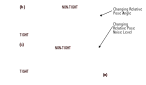
\includegraphics[width=\columnwidth]{figs/stereo_angle_study}
	\caption{Investigation of effect of pose interactions on tightness boundaries for two-pose localization with a stereo-camera model (parameters in body text). Boundaries indicates where the (smoothed) minimum \rev{ER } exceeds $ 10^{7}$ across 10 trials (without redundant constraints) and a diagram of the scenario is shown in (a). (b) shows the effect of observing the landmarks from a second pose at different vantage points, parameterized by the angle between poses. Noise level is fixed to 0.1 m and 0.1 rad. (c) Shows the effect of fixing the angle to 45 deg and varying the level of relative-pose noise (standard deviation in legend is equal for trans. and rot.).}
	\label{fig:stereo_angle}
\end{figure}

\subsubsection{Experiment in a Controlled Environment}

To assess tightness of stereo localization, we use the same setup as in Section \ref{sec:stereoslam_starry} randomly select 30 poses from the dataset and solve the SDP relaxation with and without redundant constraints. We add relative-pose measurements between subsequent poses based on the ground-truth data and perturb these measurements by a controlled amount of (isotropic) noise allowing to assess the effect of these additional measurements. 

Figure \ref{fig:d3_loc_box} shows the effect of adding redundant constraints on the \rev{ER } (tightness) of the localization problem. When there are no restrictions on the pose selection (Figure \ref{fig:d3_loc_box}(a)), it is clear that adding redundant constraints is required to obtain tightness for reasonable noise levels. When poses are restricted so that they observe at least 15 landmarks each (Figure \ref{fig:d3_loc_box}(b)), we see that, without redundant constraints, the problem is tight for higher levels of relative-pose noise and, with redundant constraints, the problem is tight across \emph{all noise levels}. This is consistent with the observations in Section \ref{sec:NoiseAnalysis}.


\begin{figure}[!b]
	\centering
	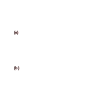
\includegraphics[width=\columnwidth]{figs/loc_box_plots}
	\caption{\rev{ER } results with and without redundant constraints for localization on random selections of 30 poses from the ``Starry Night'' dataset with relative-pose measurements between subsequent poses. 10 trials (random selection of poses) were performed at each noise level. (a) shows results when any pose can be selected, regardless of number of landmarks observed. (b) shows results when pose selection is restricted to poses that observe more than 15 landmarks.}
	\label{fig:d3_loc_box}
\end{figure}
